%iffalse
\let\negmedspace\undefined
\let\negthickspace\undefined
\documentclass[journal,12pt,onecolumn]{IEEEtran}
\usepackage{cite}
\usepackage{amsmath,amssymb,amsfonts,amsthm}
\usepackage{algorithmic}
\usepackage{graphicx}
\usepackage{textcomp}
\usepackage{xcolor}
\usepackage{txfonts}
\usepackage{listings}
\usepackage{enumitem}
\usepackage{mathtools}
\usepackage{gensymb}
\usepackage{comment}
\usepackage[breaklinks=true]{hyperref}
\usepackage{tkz-euclide} 
\usepackage{listings}
\usepackage{booktabs}
\usepackage{pgfplots}
\usepackage{gvv}                                        
%\def\inputGnumericTable{}                                 
\usepackage[latin1]{inputenc}     
\usepackage{xparse}
\usepackage{color}                                            
\usepackage{array}                                            
\usepackage{longtable}                                       
\usepackage{calc}                                             
\usepackage{multirow}
\usepackage{multicol}
\usepackage{hhline}                                           
\usepackage{ifthen}                                           
\usepackage{lscape}
\usepackage{tabularx}
\usepackage{array}
\usepackage{float}
\newtheorem{theorem}{Theorem}[section]
\newtheorem{problem}{Problem}
\newtheorem{proposition}{Proposition}[section]
\newtheorem{lemma}{Lemma}[section]
\newtheorem{corollary}[theorem]{Corollary}
\newtheorem{example}{Example}[section]
\newtheorem{definition}[problem]{Definition}
\newcommand{\BEQA}{\begin{eqnarray}}
\newcommand{\EEQA}{\end{eqnarray}}
\newcommand{\define}{\stackrel{\triangle}{=}}
\theoremstyle{remark}
\newtheorem{rem}{Remark}
% Marks the beginning of the document
\begin{document}



\bibliographystyle{IEEEtran}
\vspace{3cm}


\title{2018-CE-'14-26'}
\author{EE24BTECH11023}
%\maketitle
%\newpage
%\bigskip

{\let\newpage\relax\maketitle}

\renewcommand{\thefigure}{\theenumi}
\renewcommand{\thetable}{\theenumi}
\setlength{\intextsep}{10pt} % Space between text and floats


\numberwithin{equation}{enumi}
\numberwithin{figure}{enumi}
\renewcommand{\thetable}{\theenumi}

\begin{enumerate}
  
\item A bitumen sample has been graded as VG30 as per IS: 73-2013. The '30' in the grade means that
    \begin{enumerate}
        \item penetration of bitumen at $25^{\circ}C$ is between 20 and 40
        \item viscosity of bitumen at $60^{\circ}C$ is between 2400 and 3600 Poise
        \item ductility of bitumen at $60^{\circ}C$ is more than 30 cm
        \item elastic recovery of bitumen at $60^{\circ}C$ is more than 30\%
    \end{enumerate}

\item The speed-density relationship for a road section is shown in the figure.\\

  \begin{figure}[H]
        \centering
        
    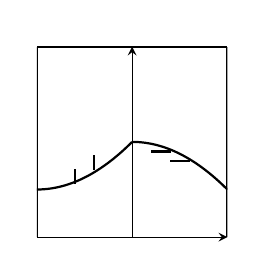
\begin{tikzpicture}
        \begin{axis}[
            axis lines = middle,
            xlabel = $ $,
            ylabel = $ $,
            xmin = -0.5, xmax = 0.5,
            ymin = 0, ymax = 1,
            xtick = {0},
            ytick = {0},
            x label style={at={(axis description cs:1,0)},anchor=west},
            y label style={at={(axis description cs:0,1)},anchor=south},
            extra tick style={grid=major},
            width=4cm, height=4cm,
            samples=100,
            domain=-0.5:0.5,
        ]
                \addplot[domain=-0.5:0, samples=100, thick] {0.25+(x+0.5)^2};
\draw [thick](-0.5,0) -- (-0.5,1);
\draw [thick](0.5,0) -- (0.5,1);
\draw [thick](0.5,1) -- (-0.5,1);
                \addplot[domain=0.1:0.2, samples=100, thick] {0.45};
                \addplot[domain=0.2:0.3, samples=100, thick] {0.40};
             \draw [thick](-0.2,0.35) -- (-0.2,0.43);
                          \draw [thick](-0.3,0.28) -- (-0.3,0.36);





        \addplot[domain=0:0.5, samples=100, thick] {0.5-x^2};



        \end{axis}
    \end{tikzpicture}
    
  % Use the correct path to your Q4.tex file
    \end{figure}
       
The shape of the flow-density relationship is
    \begin{enumerate}
        \item piecewise linear
        \item parabolic
        \item initially linear then parabolic
        \item initially parabolic then linear
    \end{enumerate}

\item A well-designed signalized intersection is one in which the
    \begin{enumerate}
        \item crossing conflicts are increased
        \item total delay is minimized
        \item cycle time is equal to the sum of red and green times in all phases
        \item cycle time is equal to the sum of red and yellow times in all phases
    \end{enumerate}

\item A flow field is given by $u = y^2$, $v = -xy$, $w = 0$. Value of the z-component of the angular velocity (in radians per unit time, up to two decimal places) at the point (0, -1, 1) is \underline{\hspace{1cm}}


\item The frequency distribution of the compressive strength of 20 concrete cube specimens is given in the table.
  \begin{table}[H]
        \centering
        
    \begin{tabular}{cc}
        \toprule
        \( f \) (MPa) & Number of specimens with \\
                      & compressive strength equal to \( f \) \\
        \midrule
        23   & 4 \\
        28   & 2 \\
        22.5 & 5 \\
        31   & 5 \\
        29   & 4 \\
        \bottomrule
    \end{tabular}
  % Use the correct path to your Q4.tex file
    \end{table}
       
    If $\mu$ is the mean strength of the specimens and $\sigma$ is the standard deviation, the number of specimens (out of 20) with compressive strength less than $\mu - 3\sigma$ is \underline{\hspace{1cm}}

\item In a fillet weld, the direct shear stress and bending tensile stress are 50 MPa and 150 MPa, respectively. As per IS 800:2007, the equivalent stress (in MPa, up to two decimal places) will be \underline{\hspace{1cm}}

\item In a shrinkage limit test, the volume and mass of a dry soil pat are found to be 50 cm$^3$ and 88 g, respectively. The specific gravity of the soil solids is 2.71, and the density of water is 1 g/cc. The shrinkage limit (in \%, up to two decimal places) is \underline{\hspace{1cm}}

\item A core cutter of 130 mm height has inner and outer diameters of 100 mm and 106 mm, respectively. The area ratio of the core cutter (in \%, up to two decimal places) is \underline{\hspace{1cm}}

\item A 1:50 model of a spillway is to be tested in the laboratory. The discharge in the prototype spillway is 1000 m$^3$/s. The corresponding discharge (in m$^3$/s, up to two decimal places) to be maintained in the model, neglecting variation in acceleration due to gravity, is \underline{\hspace{1cm}}

\item A 10 m wide rectangular channel carries a discharge of 20 m$^3$/s under critical condition. Using $g = 9.81 \, \text{m/s}^2$, the specific energy (in m, up to two decimal places) is \underline{\hspace{1cm}}

\item For routing of flood in a given channel using the Muskingum method, two of the routing coefficients are estimated as $C_0 = -0.25$ and $C_1 = 0.55$. The value of the third coefficient $C_2$ would be \underline{\hspace{1cm}}

\item A city generates $40 \times 10^6$ kg of municipal solid waste (MSW) per year, out of which only 10\% is recovered/recycled and the rest goes to landfill. The landfill has a single lift of 3 m height and is compacted to a density of 550 kg/m$^3$. If 80\% of the landfill is assumed to be MSW, the landfill area (in m$^2$, up to one decimal place) required would be \underline{\hspace{1cm}}\\

\begin{large}

\text{Q.26-Q.55 Carry two marks each}
\end{large}

\item The value of the integral $\int_{0}^{\pi} x \cos^2 x \, dx $ is
\begin{multicols}{4}

    \begin{enumerate}
        \item $\frac{\pi^2}{8}$
        \item $\frac{\pi^2}{4}$
        \item $\frac{\pi^2}{2}$
        \item $\pi^2$
    \end{enumerate}
\end{multicols}
\end{enumerate}

\end{document}
